\documentclass[a4paper, 12pt]{report}
\usepackage[english]{babel}
\usepackage{multirow}
\usepackage{wrapfig}		%wrapping figure
\usepackage[utf8]{inputenc}
\usepackage[T1]{fontenc}
\usepackage[dvipdfm]{hyperref}
\usepackage{makeidx}
\usepackage{graphicx}
\usepackage{capt-of}
\usepackage[all]{hypcap}	%ref figure correct
\usepackage[table]{xcolor}	%color table
%\newcommand{\argmax}{\mathop{\mathrm{arg\,max}}}
%\usepackage{mathtools}
\usepackage{amsmath}		% equation

%I define the measures of the document
\oddsidemargin -1.2cm
\headsep -2.4cm
\textwidth=17.0cm
\textheight=26cm

\setcounter{tocdepth}{3}


\begin{document}

%Title of the report
\title{\textbf{Czech Cities}}
%Name Of the Author
\author{\textbf{Luis Ildefonso Gómez Solana}}
%Create a title
\maketitle
%Create a index
\tableofcontents

%Create first chapter
\chapter{Czech Republic}
%Create sections
\section{Something about Czeck Republic.}
	\textbf{Czech} short from  \emph{Česko} is a landlocked country in \textbf{Central Europe}. The country is bordered by Poland to the north, Germany to the west, Austria to the south and Slovakia to the east. Its capital and largest city, with 1.3 million inhabitants, is Prague.


	It is a pluralist multi-party parliamentary representative democracy, a member of the European Union, NATO, the OECD, the OSCE, the Council of Europe and the Visegrád Group.


	\textbf{The Czech state}, formerly \textbf{known as Bohemia}, was formed in the late 9th century as a small duchy around Prague, at that time under dominance of the powerful Great Moravian Empire. After the fall of the Empire in 907, the centre of power was transferred from Moravia to Bohemia, under the Přemyslids. During the rule of Přemyslid dukes/kings and their successors, the Luxembourgs, the country reached its greatest territorial extent (13th–14th century). Life in the country was significantly affected by the Hussite wars, during which it faced economic embargo and crusades from all over Europe. The Crown of Bohemia was gradually integrated into the Habsburg monarchy as one of its three principal parts alongside the Archduchy of Austria and the Kingdom of Hungary. The Bohemian Revolt (1618–20) led to the further centralization of the monarchy. During radical reforms in the 18th century the Bohemian Crown was even de facto abolished (1749). In the 19th century the Czech lands became the industrial powerhouse of the monarchy and the core of the Republic of Czechoslovakia which was formed in 1918, following the collapse of the Austro-Hungarian empire after World War I.
\begin{wrapfigure}{r}{0.35\textwidth}
	\begin{center}
		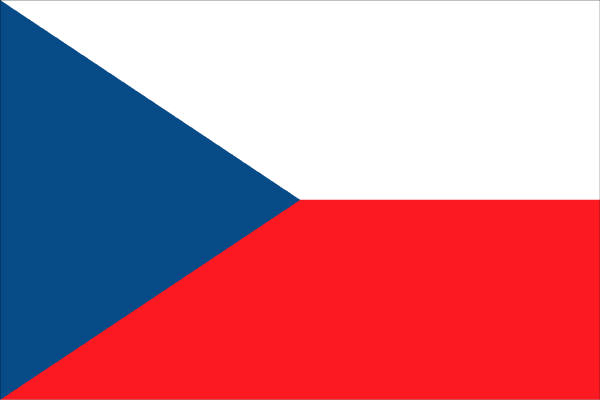
\includegraphics[width=0.25\textwidth]{cz.jpg}
	\end{center}
	\caption{Czech Republic's flag}
\end{wrapfigure}

	After the Munich Agreement, Polish annexation of Zaolzie and German occupation of Czechoslovakia and the consequent disillusion with the Western response and gratitude for the liberation of the major portion of Czechoslovakia by the Red Army, the Communist Party of Czechoslovakia won the majority in the 1946 elections. 
	In 1968, the increasing dissatisfaction culminated in attempts to reform the communist regime. The events, known as the Prague Spring of 1968, ended with an invasion by the armies of the Warsaw Pact countries; the troops remained in the country until the 1989 Velvet Revolution, when the communist regime collapsed. On 1 January 1993, Czechoslovakia peacefully dissolved into its constituent states, the Czech Republic and the Slovak Republic.

\newpage
\subsection{Images: Where is Czech Republic}
Their flag, how is the size of this country and where it is in europe.
	\begin{figure}[h] %para here [b] para bottom [t] para top
		\begin{center}
		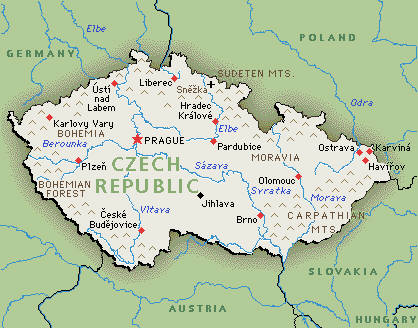
\includegraphics[width=200pt]{czech-republic.jpg}
		\caption{Country}
		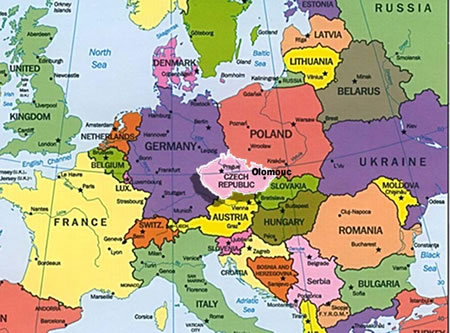
\includegraphics[width=200pt]{Europe_map.jpg}
		\caption{Europe map}
		\end{center}
	\end{figure}

\newpage
\chapter{Cities}
\section{What cities you have to visit.}

If you decide to come here, you will should visit all of this cities. So now, we will explain you a bit information that you need to know. Cities:
\begin{itemize}
	\item {\href{ttp://whc.unesco.org/en/list/616}{Prague}.} (\ref{praha})
	\item {\href{http://www.ceskatelevize.cz/ct24/regiony/122069-hradec-kralove-chce-byt-na-seznamu-unesco/}{Hradec Kralove}.} (\ref{hradec})
\end{itemize}

Moreover, you can check for this cities with UNESCO monuments inside too:
	\begin{table}[h]
		\begin{center}	
		\rowcolors{2}{gray}{white}
		\begin{tabular}{|c|c|c|}
		\rowcolor{orange}
		\hline
		City & Distance from Prague by car (km) & Web-page \\
		\hline
		Kutná Hora & 86 & \href{http://www.kutnahora.cz/index.php?lns=en}{kutnahora.cz}\\
		\hline
		Litomyšl & 170 & \href{http://whc.unesco.org/en/list/901}{whc.unesco.org/litomysl}\\
		\hline
		Olomuc & 283 & \href{http://www.olomouc.eu/portal/aktuality}{olumuc.eu}\\
		\hline
		Kroměříž & 271 & \href{http://whc.unesco.org/en/list/860}{whc.unesco.org/kromeriz}\\
		\hline
		Brno & 209 & \href{http://www.brno.me/}{brno.me}\\
		\hline
		České Budějovice & 157 & \href{http://www.c-budejovice.cz/stranky/magistrat-mesta-ceske-budejovice.aspx}{www.c-budejovice.cz}\\
		\hline
		Lednice-Valtice Area & 263 & \href{http://en.czech-unesco.org/lednice-valtice-cultural-landscape/introduction/}{en.czech-unesco.org}\\
		\hline
		\end{tabular}
		\caption{Prague information}
		\end{center}
	\end{table}

You will obtain more information into \href{unesco.org}{UNESCO Website}.


% section
\newpage
	\subsection{Prague.} \label{praha}
	Prague is the capital of the Czech Republic and fourteenth largest city in European Union. 


	Prague has been a political, cultural, and economic centre of central Europe with waxing and waning fortunes during its 1,100 year existence. It was an important city previously and after World War I became the capital of Czechoslovakia. The city played major roles in the Protestant Reformation, the Thirty Years' War, and in modern history generally as the principal conurbation in Bohemia and Moravia.

	\begin{table}[h]
		\begin{center}	
		\begin{tabular}{|c|c|}
		\hline
		  & Prague \\
		\hline
		 Population & 1,262,106 \\
		\hline
		 Density & 2,500 $km^{2}$ \\
		\hline
		\end{tabular}
		\caption{Prague information}
		\end{center}
	\end{table}

	In addition, the most important places that you have to visit in Prague are Charles Bridge (See figure \ref{fig:bridge}) and Prague Castle (See figure \ref{fig:castle})


	\subsubsection{Pictures of Prague}
		\begin{figure}[h] %h means here!
			\centering
			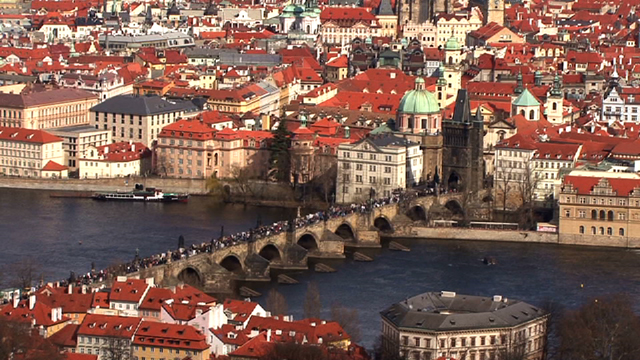
\includegraphics[width=150pt]{prague.jpg}
			\caption{Charles Bridge}	%label to make references
			\label{fig:bridge}
		\end{figure}
		\begin{figure}[h] %h means here!
			\centering
			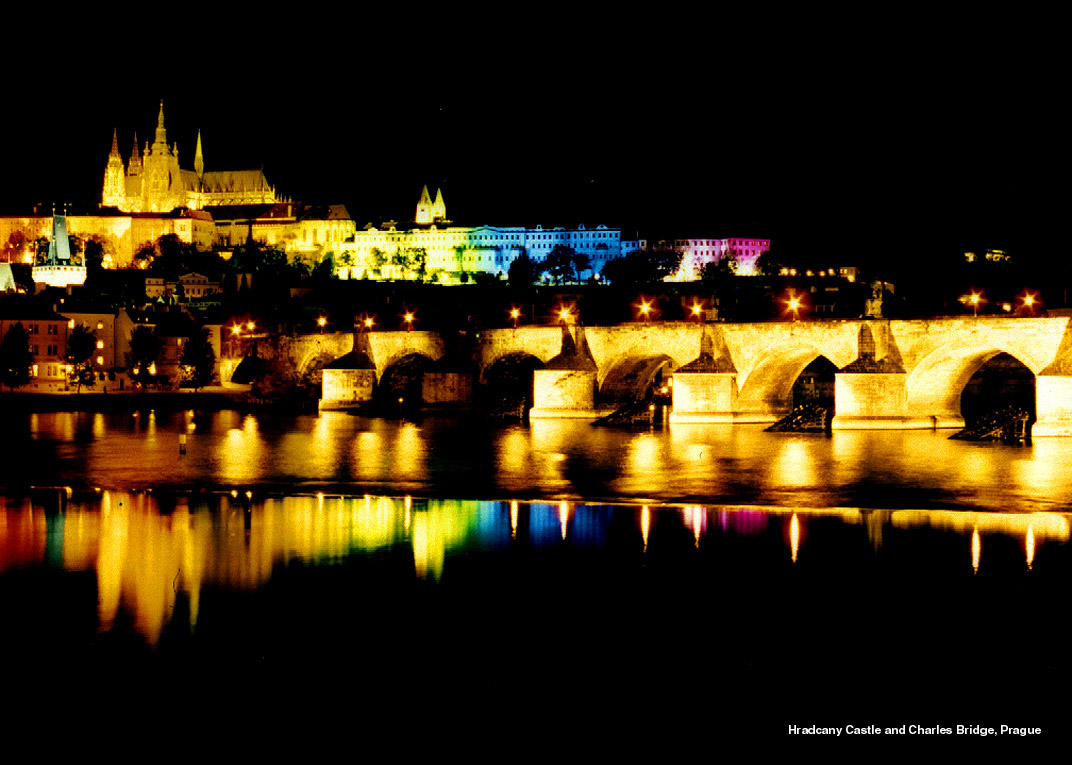
\includegraphics[width=150pt]{PragueCastleAtNight.jpg}
			\caption{\label{fig:castle}Prague Castle at night} 	%label to make references
			\label{fig:castle}
		\end{figure}
%end prague


% section
\newpage
	\subsection{Hradec Kralove.} \label{hradec}
Hradec Králové is a city of the Czech Republic, in the Hradec Králové Region of Bohemia. The city's economy is based on food-processing technology, photochemical, and electronics manufacture. Traditional industries include musical instrument manufacturing – the best known being PETROF pianos. The University of Hradec Králové is located in the city, and Charles University in Prague has a medical school and a pharmaceutical department there.

	\begin{table}[h]
		\begin{center}	
		\begin{tabular}{|c|c|}
		\hline
		  & Prague \\
		\hline
		 Population & 94,255 \\
		\hline
		 Density & 892 $km^{2}$ \\
		\hline
		\end{tabular}
		\caption{Prague information}
		\end{center}
	\end{table}

	Hradec Kralove was mentioned like natural paradise by UNESCO. You can see pictures below \ref{fig:kralove}.


	\subsubsection{Pictures of Hradec Kralove}
		\begin{figure}[h] %h means here!
			\centering
			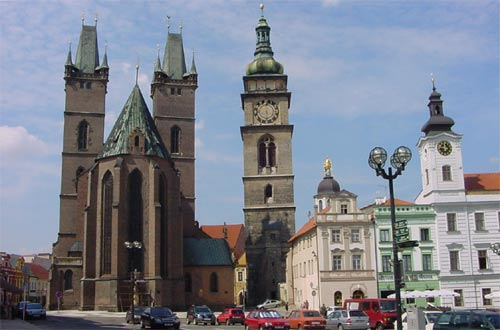
\includegraphics[width=150pt]{hradeckralove_v.jpg}
			\caption{\label{fig:kralove} Hradec Kralove}	%label to make references
		\end{figure}
%end hradec kralove

\newpage
\chapter{Formula}
\section{Calculate your trip!}
	Now you can calculate the cost of all of your trips with this formula:
		\begin{equation}
			\alpha = \sum_{i=0}^{n} (\beta) \cdot \frac {log(\gamma )}{\delta}  + x * (50)
		\end{equation}
	Where:
	\begin{enumerate}
		\item  $\beta$: kilometres between Prague and the city.
		\item \emph{n}: Each city that you want to visit.
		\item $\gamma$: Weather coefficient. If it is perfect, it will be 1. e.o.c. it will be 0 (See this \href{http://www.weather.com/weather/tenday/Prague+Czech+Republic+EZXX0012}{website}).
		\item $\delta$: How many crons are one euro (See this \href{http://themoneyconverter.com/EUR/SEK.aspx}{website}).
		\item \emph{x}: Days. It will be multiplicate by 50 euros for food.
	\end{enumerate}

	After that, you can know how much euros your trip will cost you. You have to know that it is possible to rent a car or go by train too. So please, check all of your possibilities!
\newpage
\begin{thebibliography}{9}
	% Bibliografia
	\bibitem{en.wikipedia}\href{http:\\en.wikipedia.org/wiki/Prague}{en.wikipedia.org/wiki/Prague}
	\bibitem{es.wikipedia}\href{http:\\es.wikipedia.org/wiki/Prague}{es.wikipedia.org/wiki/Prague}
	\bibitem{PragueTourism}\href{http:\\www.pragueexperience.com/information/tourism.asp}{www.pragueexperience.com/information/tourism.asp}
	\bibitem{DiscoverPrague}\href{http:\\www.discoverczech.com/apictures/z_hradeckralove/hradec-kralove/}{www.discoverczech.com}
\end{thebibliography}
\end{document}
